\documentclass[11pt]{article}
\usepackage[a4paper,margin=25mm]{geometry}
\usepackage[T1]{fontenc}
\usepackage{lmodern,microtype,amsmath,amssymb,amsthm,mathtools,graphicx,booktabs,array}
\usepackage[dvipsnames]{xcolor}
\usepackage{enumitem}
\usepackage[colorlinks=true,linkcolor=MidnightBlue,citecolor=MidnightBlue,urlcolor=MidnightBlue]{hyperref}
\usepackage[capitalise,noabbrev]{cleveref}
\usepackage{fancyhdr}
\pagestyle{fancy}\fancyhf{}\lhead{\small Phase-compatible spectral flux}\rhead{\small Shivam Gupta}\cfoot{\thepage}
\setlength{\headheight}{14pt}
\newtheorem{theorem}{Theorem}[section]
\newtheorem{proposition}[theorem]{Proposition}
\newtheorem{corollary}[theorem]{Corollary}
\newtheorem{remark}[theorem]{Remark}
\newcommand{\T}{\mathbb T}\newcommand{\Z}{\mathbb Z}\newcommand{\R}{\mathbb R}
\newcommand{\PiE}{\Pi_E}\newcommand{\PiZ}{\Pi_Z}\newcommand{\norm}[1]{\left\lVert#1\right\rVert}
\title{Phase-compatible bounds for instantaneous spectral flux\\in two-dimensional Euler flow}
\author{Shivam Gupta\\\small Independent Researcher, Delhi, India\\\small\href{mailto:shivam1720406@gmail.com}{shivam1720406@gmail.com}}
\date{17 October 2026}
\begin{document}
\maketitle
\begin{abstract}
Bounding each Fourier triad independently need not give an attainable bound on fluid energy transfer: triads sharing modes inherit exact phase relations. We formulate this compatibility constraint for instantaneous spectral flux in two-dimensional incompressible Euler flow. An integer left-nullspace criterion characterizes when the independent-triad bound is attained. For a four-triad cycle, a sharp phase optimization reduces to maximizing the sum of two square roots of affine functions on $[-1,1]$. A six-mode, real-valued initial condition realizes a strict gap; an explicit algebraic amplitude choice makes the attainable maximum $1/\sqrt2$ times the independent-triad bound. We then combine sharp four-cycle penalties with general integer-relation penalties to produce rationally checkable upper bounds for larger Fourier supports. Across twelve declared finite-support conditions, the method improves eight bounds, by $0.048$--$2.461\%$, and leaves four unchanged. Separate convolution and physical-space calculations agree with grouped flux formulas within $3.4\times10^{-15}$ across 600 evaluations. A further 624 coefficient configurations verify constructive attainment of the four-cycle formula. The result is a certificate-producing method for finite-support instantaneous flux, with applications to reproducible solver and surrogate benchmarks; it does not predict statistical cascade direction or certify a time-dependent turbulent trajectory.
\end{abstract}
\noindent\textbf{Keywords:} two-dimensional Euler equations; spectral flux; triad phases; constructive bounds; exact arithmetic; computational verification.\\
\textbf{Code and data:} \url{https://github.com/shi1720/triad-flux}

\section{Introduction}
The nonlinear term in an incompressible fluid redistributes energy among Fourier modes. Bounding the magnitude of each interacting triad and adding the results gives a simple estimate of spectral transfer. This operation forgets that the phases of different triads can depend on the same Fourier coefficients. The neglected constraint is kinematic: a prescribed list of individually favorable triad phases need not be realizable by any real velocity field with the specified Fourier amplitudes.

The distinction matters when a maximum transfer is used to normalize a numerical observation, design an extreme initial condition, or test a reduced model. An upper bound remains valid when it ignores compatibility, but it can overstate the available transfer even before dynamics, viscosity, or statistical assumptions enter. A constructive study should identify both an obstruction and an initial field attaining the corrected maximum.

We consider the nonlinear flux through a circular Fourier cutoff on $\T^2$, at an instant when the vorticity has a declared finite support. This is an exact initial-data question for the full Euler equation. The support is not assumed invariant under subsequent evolution. Our contributions are: (i) an attainability criterion expressed through integer relations among triad phase rows; (ii) a sharp four-triad reduction and an explicit Euler initial condition with a $29.289\%$ gap from the independent-triad estimate; and (iii) a composable certificate construction, implemented with rational arithmetic and independently checked on larger supports. The general integer-relation estimate also detects incompatibility in cases where four-row searches find none.

These are specialized constructive results. The underlying Fourier transfer identity, integer linear algebra, and frustrated-cycle optimization are established tools. The contribution is their combination into fluid-specific, reproducible flux certificates, with exact examples, attaining fields, and an explicit distinction between proof and numerical evidence.

\section{Relation to prior work}
The dual-cascade picture of two-dimensional turbulence is grounded in the simultaneous conservation of energy and enstrophy \cite{kraichnan}. It concerns transfer across scales under dynamical and statistical conditions, whereas our optimization holds amplitudes fixed at one instant.

Fourier phase dynamics already provide an established explanation of transfer efficiency. Murray and Bustamante \cite{murray} study synchronization, intermittency, and a fixed-amplitude phase model in Burgers turbulence. Protas, Kang, and Bustamante \cite{protas} examine triad alignment in Burgers flows arising from extreme finite-time enstrophy-growth initial data. More directly, Benavides and Bustamante \cite{benavides} develop a stochastic triad-phase closure for two-dimensional turbulence and infer cascade directions. Our question concerns joint realizability of extremal phases for a specified finite field. A deterministic dependence among several phases does not imply strong pairwise correlations; the present result therefore does not contradict the approximate weak-correlation regime used in that closure.

Harper, Bustamante, and Nazarenko \cite{harper} encode interacting triads by an integer cluster matrix and use its nullspace to identify quadratic invariants of wave clusters. We use the integer \emph{left} kernel of a phase map to constrain simultaneous transfer targets. This is a different functional of the same kind of incidence data. The equal-weight four-cycle problem is mathematically the frustrated square of an XY model; its noncollinear optimum is classical \cite{diep}. We give the weighted reduction to make the fluid certificate self-contained, not to claim a new spin-model ground state.

Geometric constraints on transfer have also been studied in physical space. Ballouz and Ouellette \cite{ballouz} analyze stress--strain eigenframe alignment and normalized cascade efficiency. Here the geometry is the shared-mode phase constraint of a Fourier polynomial. Finally, learned fluid solvers provide a concrete computational context in which physically constrained benchmarks are useful \cite{kochkov}. We evaluate the certificate itself, rather than a learned solver or a commercial deployment.

\section{Flux as a compatible cosine polynomial}\label{sec:setup}
Let $x\in(\R/2\pi\Z)^2$ and use the normalized spatial mean. Write
\begin{equation}\label{eq:pde}
 \partial_t\omega+u\cdot\nabla\omega=0,\qquad
 \nabla\cdot u=0,\qquad
 \widehat u_k=\frac{i(k_y,-k_x)}{|k|^2}\widehat\omega_k\quad(k\ne0).
\end{equation}
Thus $\partial_xu_y-\partial_yu_x=\omega$. The vorticity is real and mean zero. At the instant of interest, $\widehat\omega_k$ is nonzero only on $S\cup(-S)$, where $S$ contains one representative of each occupied pair and no zero mode. Set
\begin{equation}
 \widehat\omega_k=A_k e^{i\phi_k},\quad k\in S,\qquad
 \widehat\omega_{-k}=\overline{\widehat\omega_k},\qquad A_k>0.
\end{equation}
The Fourier equation and low-mode energy are
\begin{align}
 \partial_t\widehat\omega_k&=-\sum_{p+q=k}\frac{p\times q}{|p|^2}\widehat\omega_p\widehat\omega_q,\label{eq:fourier}\\
 E_{\le K}&=\frac12\sum_{0<|k|\le K}\frac{|\widehat\omega_k|^2}{|k|^2},\qquad
 Z_{\le K}=\frac12\sum_{0<|k|\le K}|\widehat\omega_k|^2.\label{eq:observables}
\end{align}
All sums in this paper include both signs unless specified otherwise. Positive nonlinear flux means loss from the low modes:
\begin{equation}\label{eq:flux}
 \PiE(K)=-\frac{dE_{\le K}}{dt}
 =\sum_{0<|k|\le K}\sum_{p+q=k}
 \frac{p\times q}{|k|^2|p|^2}
 \operatorname{Re}\left(\overline{\widehat\omega_k}\widehat\omega_p\widehat\omega_q\right).
\end{equation}
For enstrophy flux, omit $|k|^{-2}$ from the coefficient. No imaginary part is used with this vorticity convention. Equation~\eqref{eq:flux} follows directly by differentiating~\eqref{eq:observables} and inserting~\eqref{eq:fourier}.

Group conjugate terms and permutations with the same phase, identifying a phase row with its negative because cosine is even. After canceling zero coefficients, both observables have the form
\begin{equation}\label{eq:polynomial}
 F_c(\phi)=\sum_{e=1}^m c_e\cos(M_e\phi),\qquad M\in\Z^{m\times n},\qquad c_e\in\R\setminus\{0\}.
\end{equation}
Here $n=|S|$, and each $M_e$ is the signed row for $\phi_p+\phi_q-\phi_k$ after applying reality. The coefficient includes all relevant geometric factors and amplitudes. With integer modes and rational amplitudes, $c_e$ is rational. An interaction whose receiving mode is initially absent contributes nothing to the instantaneous quadratic flux, even if that mode has a nonzero time derivative. This explains why the finite sum describes the full equation at this instant.

Define the independent-triad estimate and the compatible maximum by
\begin{equation}
 B(c)=\sum_e|c_e|,\qquad C(M,c)=\max_{\phi\in\T^n}F_c(\phi)\le B(c).
\end{equation}
The torus is compact, so the maximum exists. For fluid flux, replacing $\omega$ by $-\omega$ reverses every cubic transfer while preserving amplitudes. Its attainable range is therefore symmetric, with extrema $\pm C(M,c)$. Translating the field changes $\phi_k$ by $k\cdot x_0$ and leaves every triad phase unchanged.

\section{Attainability and quantitative obstructions}\label{sec:criterion}
Let $b_e=0$ for $c_e>0$ and $b_e=1$ for $c_e<0$. Each summand attains $|c_e|$ precisely when $(M\phi)_e=\pi b_e$ modulo $2\pi$.

\begin{theorem}[Exact compatibility criterion]\label{thm:criterion}
For the polynomial~\eqref{eq:polynomial}, $C(M,c)=B(c)$ if and only if
\begin{equation}\label{eq:parity}
 z^Tb\in2\Z\qquad\text{for every }z\in\Z^m\text{ satisfying }M^Tz=0.
\end{equation}
If a relation violates~\eqref{eq:parity}, then $C(M,c)<B(c)$.
\end{theorem}
\begin{proof}
Equality in the sum of upper bounds requires equality in every summand, hence $M\phi=\pi b$ on the torus. Necessity follows by multiplying this equation by any integer left-null vector. For sufficiency, put $UMV=D$ in Smith normal form, with $U,V$ unimodular integer matrices. In the transformed torus equation, each nonzero diagonal entry of $D$ acts surjectively on $\T$. The remaining equations require the corresponding entries of $U(\pi b)$ to vanish modulo $2\pi$. The corresponding rows of $U$ form an integer basis of the left kernel: multiplying a left-null row by $U^{-1}$ shows that its first $\operatorname{rank}M$ entries vanish. Condition~\eqref{eq:parity} is exactly the consistency condition for these remaining equations. Strictness in the incompatible case follows from compactness and continuity.
\end{proof}

Checking only a nonsaturated rational basis of the left kernel can miss a parity obstruction after basis vectors are multiplied by even denominators. The theorem quantifies over the integer kernel. A single integer witness, however obtained, is sufficient to prove incompatibility. Our general-relation implementation uses this one-sided fact and does not claim a complete integer-lattice basis.

\begin{proposition}[A computable deficit from any integer witness]\label{prop:general}
Suppose $M^Tz=0$ and $z^Tb$ is odd. Let $I=\{e:z_e\ne0\}$. Then
\begin{equation}\label{eq:weighteddeficit}
 \sum_{e\in I}c_e\cos(M_e\phi)
 \le \sum_{e\in I}|c_e|-\frac{2}{\sum_{e\in I}z_e^2/|c_e|}
 \quad\text{for every }\phi.
\end{equation}
In particular, allocating equal positive weight $h$ to each row of $I$ gives a deficit of at least $2h/\sum_{e\in I}z_e^2$.
\end{proposition}
\begin{proof}
Choose wrapped errors $\epsilon_e\in[-\pi,\pi]$ with $M_e\phi=\pi b_e+\epsilon_e$ modulo $2\pi$. The relation implies $z^T\epsilon$ is an odd multiple of $\pi$, so $|z^T\epsilon|\ge\pi$. The elementary inequality $1-\cos t\ge 2t^2/\pi^2$ on this interval and weighted Cauchy--Schwarz give
\[
 \sum_{e\in I}|c_e|(1-\cos\epsilon_e)
 \ge\frac{2}{\pi^2}\sum_{e\in I}|c_e|\epsilon_e^2
 \ge \frac{2}{\sum_{e\in I}z_e^2/|c_e|}.
\]
Subtract this deficit from $\sum_{e\in I}|c_e|$.
\end{proof}

\section{A sharp four-triad envelope}\label{sec:four}
Consider four phase rows with the relation
\begin{equation}\label{eq:cycle}
 \theta_1+\theta_3=\theta_2+\theta_4\pmod{2\pi}.
\end{equation}
The relation-constrained maximum is an upper bound if further phase relations exist, and is exact when these four phases range over the whole torus defined by~\eqref{eq:cycle}.

\begin{theorem}[Weighted cycle reduction]\label{thm:four}
For arbitrary real $c_1,c_2,c_3,c_4$, the maximum under~\eqref{eq:cycle} is
\begin{equation}\label{eq:sharp}
 H(c)=\max_{-1\le t\le1}\left\{\sqrt{a+bt}+\sqrt{d+et}\right\},
\end{equation}
where $a=c_1^2+c_3^2$, $b=2c_1c_3$, $d=c_2^2+c_4^2$, and $e=2c_2c_4$. If $be<0$, an interior maximizer, when it lies in $[-1,1]$, is
\begin{equation}\label{eq:tstar}
 t_* = \frac{e^2a-b^2d}{b^2e-e^2b}.
\end{equation}
Otherwise it suffices to compare the endpoints, with values
$|c_1\pm c_3|+|c_2\pm c_4|$. An interior candidate can be chosen whenever it exists; it is globally maximizing. These rules also cover zero coefficients through the endpoint rule.
\end{theorem}
\begin{proof}
Fix $s=\theta_1+\theta_3=\theta_2+\theta_4$. Maximizing the first pair gives
\[
 \max_x\{c_1\cos x+c_3\cos(s-x)\}=|c_1+c_3e^{-is}|=\sqrt{a+b\cos s}.
\]
The second pair gives $\sqrt{d+e\cos s}$ independently. Their sum proves~\eqref{eq:sharp}; pairwise maximizing phases provide attainment. The square-root sum is concave in $t$. When $be\ge0$ it is monotone, or constant in a degenerate case. For $be<0$, its derivative vanishes when $b/\sqrt{a+bt}=-e/\sqrt{d+et}$. Squaring introduces no sign ambiguity because $b,e$ have opposite signs; solving gives~\eqref{eq:tstar}. Concavity proves maximality. If no interior stationary point exists, the maximum is an endpoint. Endpoint radicals simplify to the stated absolute values.
\end{proof}

For numerical construction, choose $s=\arccos t$ and
\begin{align}
 \theta_1&=-\arg(c_1+c_3e^{-is}),&\theta_3&=s-\theta_1,\\
 \theta_2&=-\arg(c_2+c_4e^{-is}),&\theta_4&=s-\theta_2.
\end{align}
If a complex argument vanishes, that pair has zero objective and any split of $s$ works.

\begin{corollary}[Equal-weight frustrated cycle]\label{cor:balanced}
If $|c_i|=h>0$ and $\prod_{i=1}^4\operatorname{sign}(c_i)=-1$, then $H(c)=2\sqrt2h$, while $B(c)=4h$. The deficit is $(4-2\sqrt2)h$.
\end{corollary}
\begin{proof}
After sign changes of individual phases and shifts by $\pi$, the objective is equivalent to weights $(h,h,-h,h)$. In~\eqref{eq:sharp} this is $h[\sqrt{2-2t}+\sqrt{2+2t}]$, maximized at $t=0$.
\end{proof}
The $1/\sqrt2$ factor is the familiar frustrated-square optimum \cite{diep}. Its role here is a sharp, reusable penalty for a fluid flux polynomial.

\section{An explicit Euler initial condition}\label{sec:witness}
Take the six half-plane modes
\begin{equation}\label{eq:modes}
 \begin{array}{lll}
 a=(1,-3),&b=(1,-2),&c=(1,-1),\\
 d=(2,-5),&e=(2,-3),&f=(3,-6).
 \end{array}
\end{equation}
They satisfy $a+b=d$, $b+c=e$, $d+c=f$, and $a+e=f$. Exhausting the sums and differences among these twelve signed modes yields exactly these four noncollinear triads, up to conjugation and permutation. Collinear sums have zero interaction coefficient. Their phases are
\begin{equation}\label{eq:witnessphases}
 \begin{split}
 \theta_1=\phi_a+\phi_b-\phi_d,&\qquad\theta_2=\phi_b+\phi_c-\phi_e,\\
 \theta_3=\phi_d+\phi_c-\phi_f,&\qquad\theta_4=\phi_a+\phi_e-\phi_f.
 \end{split}
\end{equation}
These obey~\eqref{eq:cycle}. Conversely, every compatible quadruple is realized by
\begin{equation}\label{eq:construct}
 \phi_a=\phi_b=\phi_c=0,\quad
 \phi_d=-\theta_1,\quad\phi_e=-\theta_2,\quad\phi_f=-\theta_1-\theta_3.
\end{equation}
Consequently the cycle envelope is the actual phase maximum of the full Euler initial-data flux.

Use $K^2=10$, so $a,b,c$ lie inside the cutoff and $d,e,f$ lie outside. With unit vorticity amplitudes, the exact coefficients in~\eqref{eq:witnessphases} order are
\begin{equation}\label{eq:coeffwitness}
 (c_1,c_2,c_3,c_4)=\left(\frac1{145},\frac3{65},-\frac{16}{435},\frac{32}{975}\right).
\end{equation}
For example, triad $a+b=d$ has $a\times b=1$, squared lengths $10,5,29$, and contributes
$2[1/(10\cdot29)-1/(5\cdot29)]=-1/145$ to $dE_{\le K}/dt$ for aligned unit amplitudes. Its outward flux coefficient is therefore $1/145$. The other three entries follow by the same full signed-mode accounting.

The preferred phases for the four signs are $(0,0,\pi,0)$, which violate~\eqref{eq:cycle}. The sharp formula gives
\begin{equation}
 B=\frac{1156}{9425}\simeq0.122652520,\qquad
 C=B-\frac2{145}=\frac{1026}{9425}\simeq0.108859416.
\end{equation}
Here $t=1$ is optimal: sacrificing the weakest triad completely is better than distributing the phase error. The phases $(\phi_a,\ldots,\phi_f)=(0,0,0,\pi,0,0)$ attain this value.

A second choice distributes the incompatibility. Set
\begin{equation}\label{eq:balancedamps}
 (A_a,A_b,A_c,A_d,A_e,A_f)
 =\left(1,1,\frac{\sqrt{30}}{15},1,\frac{13\sqrt{30}}{174},\frac{3\sqrt{30}}{32}\right).
\end{equation}
Each geometric coefficient is multiplied by its three incident amplitudes, giving $(1,1,-1,1)/145$. Thus
\begin{equation}\label{eq:balancedvalue}
 B=\frac4{145},\qquad C=\frac{2\sqrt2}{145}\simeq0.019506394,\qquad \frac CB=\frac1{\sqrt2}.
\end{equation}
A maximizing phase vector is
\begin{equation}\label{eq:balancedphi}
 (\phi_a,\ldots,\phi_f)=(0,0,0,\pi/4,-\pi/4,-\pi/2).
\end{equation}
These data define a real, smooth vorticity field with finite Fourier support. Equation~\eqref{eq:pde} gives a divergence-free velocity. At this instant, the same nonlinear flux applies to Navier--Stokes with the specified initial field. Viscosity contributes the additional low-mode loss
\[\nu\sum_{0<|k|\le K}|\widehat\omega_k|^2.\]

\begin{figure}[tb]
 \centering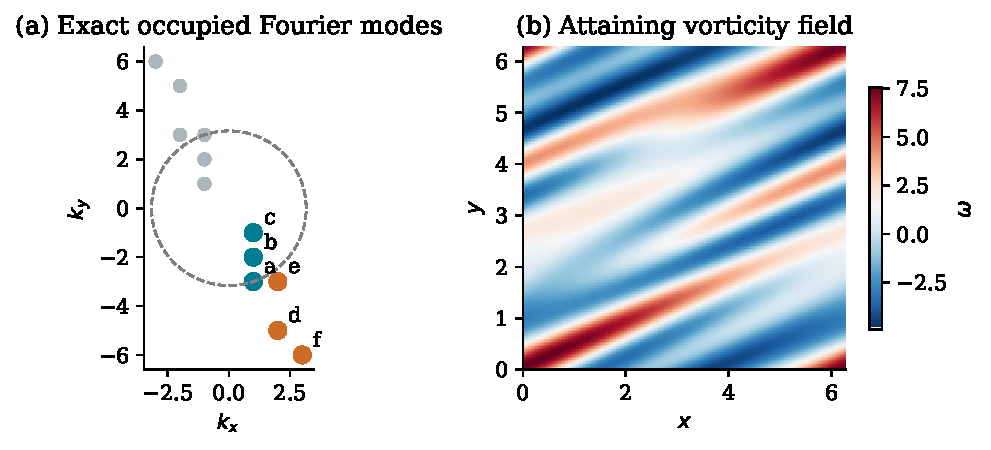
\includegraphics[width=.96\linewidth]{figures/support_witness.pdf}
 \caption{Constructed initial data. (a) Six independent modes and their conjugates; the dashed circle is $|k|^2=10$. (b) A real vorticity field attaining the balanced flux maximum. The plotted phases use an equivalent representative of the compatible phase fiber; the analytic representative is given in~\eqref{eq:balancedphi}.}
 \label{fig:witness}
\end{figure}
\begin{figure}[tb]
 \centering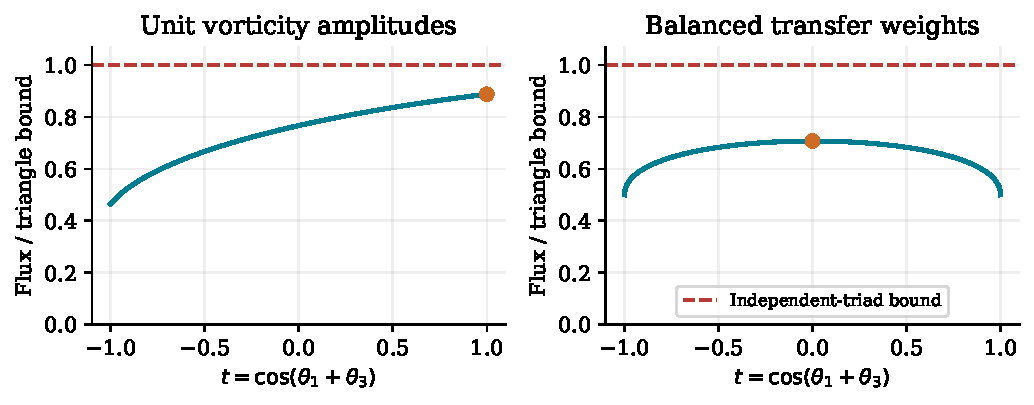
\includegraphics[width=.96\linewidth]{figures/sharp_envelopes.pdf}
 \caption{The sharp one-dimensional envelopes. Unit amplitudes place the maximum at an endpoint, while the algebraic amplitudes~\eqref{eq:balancedamps} give an interior optimum. The dashed line is the independently optimized triad sum, which is unattainable in both cases.}
 \label{fig:envelopes}
\end{figure}

\section{Composable certificates on larger supports}\label{sec:packing}
A larger flux polynomial can contain many incompatible relations. Adding the penalties from overlapping relations without an allocation rule would count the same coefficient more than once. We instead split the available magnitude of each coefficient among blocks.

For a frustrated four-row relation with entries $\pm1$, allocate equal mass $h_j\ge0$ to its four participating coefficients, retaining their original signs. Replacing $\theta_e$ by $\pm\theta_e$ puts the relation in the form~\eqref{eq:cycle}, and cosine is unchanged. Corollary~\ref{cor:balanced} gives a loss $(4-2\sqrt2)h_j$. For a general integer relation $z^{(j)}$ with odd sign parity, the same equal-mass allocation gives a loss $2h_j/\norm{z^{(j)}}_2^2$ by Proposition~\ref{prop:general}.

\begin{theorem}[Packing bound]\label{thm:packing}
Let $\mathcal Q$ be a collection of frustrated four-row $\pm1$ relations, and $\mathcal G$ any collection of odd-parity integer relations. If
\begin{equation}\label{eq:capacity}
 \sum_{j:e\in\operatorname{supp}z^{(j)}}h_j\le|c_e|\qquad(e=1,\ldots,m),
\end{equation}
then every mode phase vector satisfies
\begin{equation}\label{eq:packing}
 F_c(\phi)\le B(c)-(4-2\sqrt2)\sum_{j\in\mathcal Q}h_j
 -\sum_{j\in\mathcal G}\frac{2h_j}{\norm{z^{(j)}}_2^2}.
\end{equation}
\end{theorem}
\begin{proof}
Decompose each coefficient into the same-sign block allocations and a residual of nonnegative magnitude, permitted by~\eqref{eq:capacity}. Apply the appropriate block bound to each allocated polynomial and the absolute-value bound to the residual. Sum the inequalities.
\end{proof}

The implementation first finds four-row relations by hashing signed pair sums of phase rows. It sorts frustrated relations by decreasing minimum initial coefficient magnitude, with lexicographic ties, and allocates the minimum remaining magnitude on each block. It then computes an exact rational left-nullspace basis, clears denominators, reduces each vector to primitive integer entries, and retains odd-parity witnesses. These are sorted by their available initial penalty, followed by lexicographic ties, and allocated greedily. The basis witnesses need not include every obstruction. Neither the discovery order nor the allocation is claimed optimal.

The certificate contains $M$, rational $c$, the relation vectors, and rational allocated masses. A separate standard-library checker verifies the integer relations, parity, capacities, and penalty sums. It bounds $\sqrt2$ using integer square roots at denominator $10^{30}$, so the reported bound can be enclosed from above without trusting floating-point rounding. It checks the inequality for the supplied cosine polynomial; separate convolution and physical-space checks test its derivation from the fluid equation. This separation makes the scope of the verification explicit.

\section{Computational evaluation}\label{sec:experiments}
\subsection{Protocol and independent checks}
All experiments use seed 20261017 and are reproduced by \texttt{run\_experiments.py}. Exact coefficient discovery and certificate verification use rational arithmetic; optimization and time integration use double precision. The saved environment records Python~3.12.14, NumPy~2.5.4, SciPy~1.18.1, SymPy~1.14.0, and Matplotlib~3.11.2.

We compare the grouped polynomial to two separate evaluators: direct complex convolution of~\eqref{eq:fourier}, and physical-space multiplication $-u\cdot\nabla\omega$ on a Fourier grid. The latter uses the strict two-thirds mask for time integration. The initial witness fits comfortably within every tested grid. We use 100 independent phase/amplitude draws for each of three grids ($40^2$, $48^2$, $64^2$) and two observables, giving 600 comparisons. Amplitudes are rational draws from $\{1,\ldots,24\}/13$; phases are uniform on $[-\pi,\pi]^6$. The maximum grouped/direct difference is $1.56\times10^{-15}$, and the maximum grouped/physical-space difference is $3.39\times10^{-15}$.

For the cycle formula we exhaust $\{-2,-1,0,1,2\}^4\setminus\{0\}$, giving 624 configurations. In each case an explicit compatible phase vector attains the formula to at most $8.89\times10^{-16}$. A 1001-point scan of the reduced interval never exceeds the formula. Attainment and global optimality are established analytically in Theorem~\ref{thm:four}; the floating-point sweep checks implementation and degeneracies. The twelve-test unit suite additionally checks full energy/enstrophy cancellation, translation invariance, viscous splitting, integer Smith-form attainability (including torsion cases), general-relation detection, and rejection of tampered certificates.

\subsection{Declared finite-support suite}
We use all nonzero signed modes in $[-L,L]^2$ for $L\in\{2,3,4\}$, with half-plane representatives ordered by $k_x$ then $k_y$. Vorticity amplitudes are $A_k=(1+|k|^2)^{-p}$ for $p\in\{0,1\}$, the cutoff is $K=L$, and both energy and enstrophy are tested. This yields twelve conditions; none are discarded. They are small, deterministic finite-support benchmarks, not inertial-range turbulence simulations.

\Cref{tab:dense} gives the independent-triad bound $B$, the hybrid certificate $U$, and a numerical lower diagnostic $L_{\rm num}$. The latter is the largest attained objective among twelve L-BFGS-B starts, each with at most 1200 iterations, and is not a proof of a global maximum or a rigorously rounded lower bound. It is included to show how much uncertainty remains. Exact certificates improve eight conditions, with relative reductions from $0.0477\%$ to $2.4606\%$. Four $L=2$ conditions are unchanged. The exact Smith-form criterion confirms attainability in those four conditions and incompatibility in the other eight. Numerical optimization also reaches the four attainable triangle estimates to floating-point accuracy.

At $L=3$, there are no frustrated four-row $\pm1$ relations in the flux polynomial found by exhaustive pair-sum matching. General integer witnesses still give a positive certified deficit. At $L=4$, the four-row search finds 28 frustrated relations for each amplitude profile and observable; the hybrid construction uses 16--20 four-row allocations plus one or two general witnesses. Certificate discovery and rational construction take approximately $0.001$--$0.14$ seconds per condition on the executing machine; these single-run timings are descriptive, not a performance benchmark.

\begin{table}[tb]
\centering\small
\caption{All twelve declared finite-support conditions. $n$ counts independent conjugate pairs; $m$ counts nonzero grouped phase terms. $U$ is the hybrid upper certificate. $L_{\rm num}$ is an optimization diagnostic. Displayed values are rounded; exact rational certificate inputs are provided with the code.}
\label{tab:dense}
\begin{tabular}{rrrlrrrrr}
\toprule
$L$&$n$&$p$&Flux&$m$&$B$&$U$&$L_{\rm num}$&Gain (\%)\\
\midrule
2&12&0&Energy&12&4.40000&4.40000&4.40000&0.000\\
2&12&0&Enstrophy&12&17.2000&17.2000&17.2000&0.000\\
2&12&1&Energy&12&0.073333&0.073333&0.073333&0.000\\
2&12&1&Enstrophy&12&0.322222&0.322222&0.322222&0.000\\
3&24&0&Energy&52&8.31385&8.28385&7.02996&0.361\\
3&24&0&Enstrophy&52&74.5538&74.4392&66.4168&0.154\\
3&24&1&Energy&52&0.030714&0.030682&0.027305&0.104\\
3&24&1&Enstrophy&52&0.295795&0.295654&0.273449&0.048\\
4&40&0&Energy&156&12.9884&12.6688&9.71881&2.461\\
4&40&0&Enstrophy&156&201.709&199.140&160.664&1.274\\
4&40&1&Energy&156&0.014706&0.014528&0.012203&1.210\\
4&40&1&Enstrophy&156&0.239700&0.238207&0.206779&0.623\\
\bottomrule
\end{tabular}
\end{table}

The remaining gap between $U$ and $L_{\rm num}$ is substantial in some cases. For example, at $L=4$, $p=0$, the energy values are approximately $12.669$ and $9.719$. This can reflect missed relations, a suboptimal allocation, or an optimization diagnostic below the true maximum. The data do not distinguish those explanations. The certificate proves a strict improvement over $B$; it does not establish the sharp maximum for these larger supports.

\begin{figure}[tb]
 \centering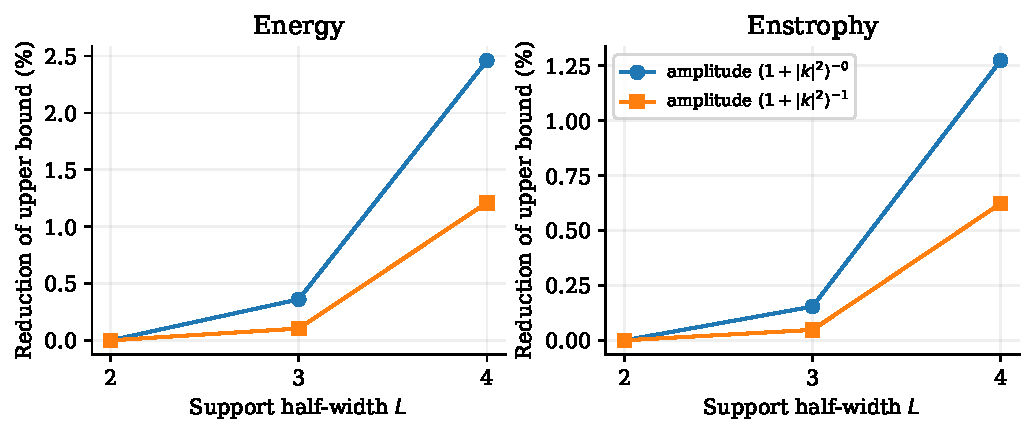
\includegraphics[width=.96\linewidth]{figures/packing_gains.pdf}
 \caption{Certified reductions relative to the independent-triad bound for the complete finite-support suite. The hybrid method detects small positive losses at $L=3$ through general integer relations, despite finding no frustrated four-row $\pm1$ relations there. Zero gains are retained.}
 \label{fig:packing}
\end{figure}

\subsection{Short-time equation checks}
Starting from the balanced maximizing initial condition, we integrate unforced Navier--Stokes with $\nu=0.01$ to $T=0.2$, using explicit RK4 and a dealiased pseudospectral nonlinearity. The four grid/step pairs are $(48,0.002)$, $(64,0.002)$, $(64,0.001)$, and $(96,0.001)$. The terminal nonlinear fluxes are respectively
$0.02014577021646$, $0.02014577022258$, $0.02014577022258$, and $0.02014577022258$. The largest difference from the last pair is $6.2\times10^{-12}$.

A separate forward difference of low-mode energy checks the sign and normalization of the initial derivative, including viscosity. Its analytic target is $0.06217306063043$. Halving the interval from $0.01$ to $0.000625$ reduces the error from $1.203\times10^{-5}$ to $6.919\times10^{-7}$, consistent with a first-order forward difference. These are numerical consistency checks. They do not enclose temporal or spectral error rigorously. The initial certificate does not bound later flux at fixed initial amplitudes: new modes and changed amplitudes appear immediately, and the later flux can exceed the initial maximum without contradiction.

\begin{figure}[tb]
 \centering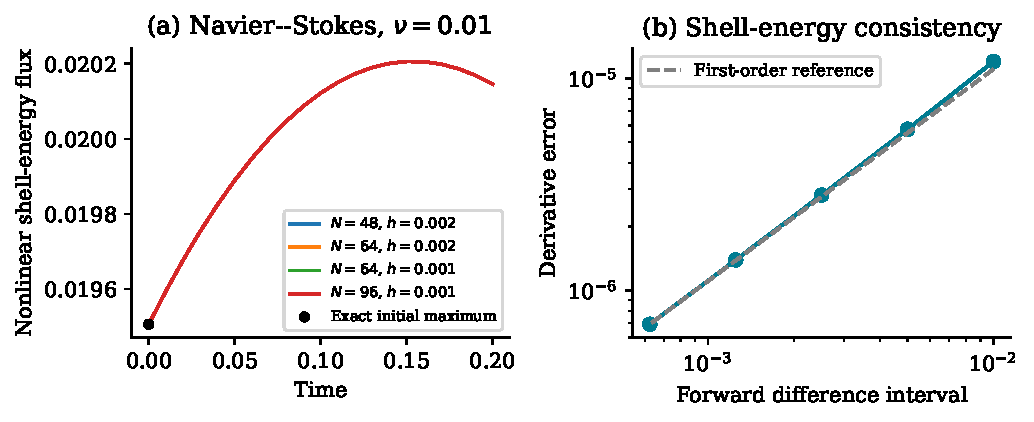
\includegraphics[width=.96\linewidth]{figures/time_checks.pdf}
 \caption{Numerical equation checks from the balanced witness. (a) Short-time nonlinear energy flux; the four curves nearly coincide at this scale. The black point is the analytically sharp initial value. (b) Forward-difference consistency of low-mode energy loss, including the known viscous term. These plots provide convergence evidence, not validated trajectory enclosures.}
 \label{fig:time}
\end{figure}

\section{Robustness, applications, and limits}\label{sec:limits}
\begin{proposition}[Coefficient perturbations]\label{prop:lipschitz}
For a fixed phase matrix and coefficient vectors $c,\widetilde c$, including zeros if necessary,
\begin{equation}
 |C(M,c)-C(M,\widetilde c)|\le\norm{c-\widetilde c}_1.
\end{equation}
Thus any certified upper bound $U$ for $c$ becomes $U+\epsilon$ for all $\widetilde c$ with $\norm{c-\widetilde c}_1\le\epsilon$.
\end{proposition}
\begin{proof}
For every $\phi$, $|F_c(\phi)-F_{\widetilde c}(\phi)|\le\norm{c-\widetilde c}_1$ because $|\cos|\le1$. Take maxima in both directions.
\end{proof}
This elementary perturbation estimate permits a conservative extension to uncertain amplitudes on the same declared finite support, once their effect on the grouped coefficients has been enclosed. If an estimated coefficient crosses zero, one should use this uniform perturbation bound rather than silently retain a sign-based relation. No amplitude-uncertainty experiment is claimed here.

A practical use is a manufactured benchmark for a spectral solver, reduced-order model, or learned fluid surrogate. The input field, its energy and enstrophy, the cutoff convention, and a sharp initial flux are all specified. A model that produces a larger nonlinear flux at those same amplitudes violates the phase-compatible constraint even if it conserves total energy. A spectrum-only generator can use the bound as a rejection test for impossible transfer targets. Learned simulation work \cite{kochkov} motivates such tests, but usefulness as a benchmark is not evidence that this test improves a trained model.

The main limitations are structural. The certificates require a declared finite support and instantaneous amplitudes. A measured or truncated field can have an unobserved tail, whose flux contribution requires an additional bound. Four-row hashing has quadratic pair storage in the number of phase terms before collisions are processed, so it is unsuitable as implemented for a large turbulent discretization. The rational basis depends on row ordering and need not supply every integer obstruction. Greedy packing can be improved and is not a global optimization of allocations. The general-relation estimate is intentionally conservative, as its $1-\cos$ inequality is not usually sharp. Neither statistical cascade direction, anomalous dissipation, nor singularity formation follows from this calculation.

Commercial relevance is correspondingly specific: the method could support verification libraries for scientific simulation or surrogate quality assurance. No customer study, economic benefit, or patentability conclusion is established. The mathematical result can stand independently of those possible applications.

\section{Conclusion}
Shared Fourier modes impose exact compatibility conditions on instantaneous transfer phases. For a declared finite-support Euler initial state, these conditions distinguish an attainable flux maximum from a sum of unattainable triad optima. A six-mode construction realizes the distinction sharply, while rationally checkable relation packings extend it to larger polynomials. The complete experiment suite shows both positive improvements and unchanged bounds. The next mathematical challenge is to make such constraints efficient and quantitatively strong for large supports and controlled unresolved tails.

\paragraph{Data and code availability.}
The repository contains source, unit tests, exact certificate data, a dependency-free verifier, all figure scripts, raw numerical checks, environment versions, and the manuscript source. Run \texttt{python run\_experiments.py}, \texttt{python -m unittest discover -s tests -v}, and \texttt{python verify\_certificates.py}. Exact analytic identities and integer/rational inequalities establish the certificates; floating-point results are labeled separately.

\begin{thebibliography}{9}\raggedright
\bibitem{kraichnan} R. H. Kraichnan. Inertial ranges in two-dimensional turbulence. \emph{Physics of Fluids}, 10:1417--1423, 1967. \href{https://doi.org/10.1063/1.1762301}{doi:10.1063/1.1762301}.
\bibitem{murray} B. P. Murray and M. D. Bustamante. Energy flux enhancement, intermittency and turbulence via Fourier triad phase dynamics in the 1D Burgers equation. \emph{Journal of Fluid Mechanics}, 850:624--645, 2018. \href{https://doi.org/10.1017/jfm.2018.454}{doi:10.1017/jfm.2018.454}.
\bibitem{protas} B. Protas, D. Kang, and M. D. Bustamante. Alignments of triad phases in extreme one-dimensional Burgers flows. \emph{Physical Review E}, 109:055104, 2024. \href{https://doi.org/10.1103/PhysRevE.109.055104}{doi:10.1103/PhysRevE.109.055104}.
\bibitem{benavides} S. J. Benavides and M. D. Bustamante. Triad phase dynamics determine cascade direction in two-dimensional turbulence. Preprint, 2026. \href{https://arxiv.org/abs/2605.03049}{arXiv:2605.03049}.
\bibitem{harper} K. L. Harper, M. D. Bustamante, and S. V. Nazarenko. Quadratic invariants for discrete clusters of weakly interacting waves. \emph{Journal of Physics A: Mathematical and Theoretical}, 46:245501, 2013. \href{https://doi.org/10.1088/1751-8113/46/24/245501}{doi:10.1088/1751-8113/46/24/245501}.
\bibitem{diep} H. T. Diep. Phase transition in frustrated magnetic thin film---physics at phase boundaries. \emph{Entropy}, 21:175, 2019. \href{https://doi.org/10.3390/e21020175}{doi:10.3390/e21020175}.
\bibitem{ballouz} J. G. Ballouz and N. T. Ouellette. Geometric constraints on energy transfer in the turbulent cascade. \emph{Physical Review Fluids}, 5:034603, 2020. \href{https://doi.org/10.1103/PhysRevFluids.5.034603}{doi:10.1103/PhysRevFluids.5.034603}.
\bibitem{kochkov} D. Kochkov, J. A. Smith, A. Alieva, Q. Wang, M. P. Brenner, and S. Hoyer. Machine learning--accelerated computational fluid dynamics. \emph{Proceedings of the National Academy of Sciences}, 118:e2101784118, 2021. \href{https://doi.org/10.1073/pnas.2101784118}{doi:10.1073/pnas.2101784118}.
\end{thebibliography}

\appendix
\section{Certificate format and verification example}\label{app:cert}
A certificate is a finite list of integer phase rows, rational coefficients, and allocated relations. For a relation written as pairs $(e,z_e)$, the checker verifies $\sum_ez_eM_e=0$ exactly and computes $\sum_{c_e<0}z_e$ modulo two. It then charges the allocated mass to each participating row. This makes overlap explicit.

For the unit-amplitude six-mode witness, the row matrix is
\[
 M=\begin{pmatrix}
 1&1&0&-1&0&0\\
 0&1&1&0&-1&0\\
 0&0&1&1&0&-1\\
 1&0&0&0&1&-1
 \end{pmatrix}.
\]
The primitive relation is $z=(1,-1,1,-1)$, and $b=(0,0,1,0)$. Hence $z^Tb=1$. An equal-weight allocation $h=1/145$ gives the valid, although nonsharp for these unequal coefficients, packing bound
\[
 U=\frac{1156}{9425}-\frac{4-2\sqrt2}{145}.
\]
The sharper weighted result in Section~\ref{sec:witness} is $B-2/145$. With the balanced amplitudes all magnitudes equal $1/145$, and the same equal-weight certificate becomes sharp. This illustrates the distinction between a correct allocated subproblem and the exact solution of the entire weighted motif.

The checker encloses the irrational term as follows. Let $N=10^{30}$ and $r=\lfloor\sqrt{2N^2}\rfloor$, computed by integer square root. Then $r/N\le\sqrt2\le(r+1)/N$. Since its coefficient in~\eqref{eq:packing} after expansion is nonnegative, substituting $(r+1)/N$ gives an exact rational upper enclosure. The difference between the upper and lower enclosures is $2\sum_{j\in\mathcal Q}h_j/N$.

\section{Reproduction details and claim boundaries}
The dense-support suite uses all nonzero modes of a square, including vertical-axis modes once in the half-plane representation. Geometric zero interactions and coefficients canceled by the complete cutoff sum are removed before counting $m$. The pair-sum search identifies all four-row $\pm1$ relations, including relations with sign patterns other than two plus and two minus; sign reversal of cosine phases preserves the four-cycle bound.

The physical-space implementation rounds FFT frequency labels to their exact integer wave numbers before computing a circular cutoff mask. Without this step, a floating-point representation of a boundary wave number can be classified on the wrong side of $|k|^2=K^2$. This implementation detail matters for the witness because $|a|^2=10$ lies on the boundary.

The analytic optimization does not require an FFT, time integrator, random initialization, or numerical optimizer. Conversely, the short-time solver has no interval-arithmetic enclosure and is not a computer-assisted proof of a PDE trajectory. The exact certificate verifier establishes inequalities for finite cosine polynomials; the proof in Section~\ref{sec:setup} connects those polynomials to finite-support instantaneous fluid flux.

The literature search covered Fourier phase synchronization and phase-only turbulence models, recent two-dimensional triad-phase closures, wave-cluster incidence matrices, physical-space transfer geometry, and frustrated XY cycles. The work claims the explicit Euler construction and the fluid-specific certificate workflow. It does not claim discovery of phase effects, of frustrated-cycle optima, or an exhaustive guarantee that no related result exists under other terminology.
\end{document}
